% ChatGPT Directions 0 : 
% This is a Tbox Problem set for the following standards: 5.NF.A.1, 5.NF.A.2
%--------------------------------------------------
\documentclass[12pt]{article}
\usepackage[a4paper, top=0.8in, bottom=0.7in, left=0.8in, right=0.8in]{geometry}
\usepackage{amsmath}
\usepackage{amsfonts}
\usepackage{latexsym}
\usepackage{graphicx}
\usepackage{fancyhdr}
\usepackage{tcolorbox}
\usepackage{enumitem}
\usepackage{setspace}
\usepackage[defaultfam,tabular,lining]{montserrat} % Font settings for Montserrat
\usepackage{tikz} % Package for visual fraction models

\setlength{\parindent}{0pt}
\pagestyle{fancy}
\setlength{\headheight}{27.11148pt}
\addtolength{\topmargin}{-15.11148pt}

\fancyhf{}
%\fancyhead[L]{\textbf{5.NF.A.1, 5.NF.A.2: Adding and Subtracting Fractions in Word Problems}}
\fancyhead[R]{
\includegraphics[width=0.8cm]{Round Logo.png}}
\fancyfoot[C]{\footnotesize © Study Smart Tutors}

\sloppy
\title{}
\date{}
\hyphenpenalty=10000
\exhyphenpenalty=10000

\begin{document}

\subsection*{Problem Set: Adding and Subtracting Fractions in Word Problems}
\onehalfspacing

% Learning Objective Box
\begin{tcolorbox}[colframe=black!40, colback=gray!5, 
coltitle=black, colbacktitle=black!20, fonttitle=\bfseries\Large, 
title=Learning Objective, halign title=center, left=5pt, right=5pt, top=5pt, bottom=15pt]
\textbf{Objective:} Solve real-world problems involving the addition and subtraction of fractions with unlike denominators, including writing and solving equations to represent these situations.
\end{tcolorbox}

% Exercises Box
\begin{tcolorbox}[colframe=black!60, colback=white, 
coltitle=black, colbacktitle=black!15, fonttitle=\bfseries\Large, 
title=Exercises, halign title=center, left=10pt, right=10pt, top=10pt, bottom=60pt]
\begin{enumerate}[itemsep=3em]

    % Model-Based Question - Numerical Answer
    \item Add the fractions represented by the models below and provide your answer as a number.

    \begin{center}
        \begin{tikzpicture}[scale=0.8]
            % Fraction Model for 3/8
            \draw[thick] (0,0) rectangle (4,0.5);
            \foreach \x in {0,1,...,7} \draw[thick] (\x*0.5,0) -- (\x*0.5,0.5);
            \foreach \x in {0,1,2} \filldraw[fill=gray!30,draw=black] (\x*0.5,0) rectangle ++(0.5,0.5);
            \node[below] at (2,-0.2) {\scriptsize Fraction Model for \( \frac{3}{8} \)};
        \end{tikzpicture}

        \vspace{0.5em}

        \begin{tikzpicture}[scale=0.8]
            % Fraction Model for 2/8
            \draw[thick] (0,0) rectangle (4,0.5);
            \foreach \x in {0,1,...,7} \draw[thick] (\x*0.5,0) -- (\x*0.5,0.5);
            \foreach \x in {0,1} \filldraw[fill=gray!30,draw=black] (\x*0.5,0) rectangle ++(0.5,0.5);
            \node[below] at (2,-0.2) {\scriptsize Fraction Model for \( \frac{2}{8} \)};
        \end{tikzpicture}
    \end{center}

    % Model-Based Question - Visual Answer
    \item Subtract the fractions represented by the models below and provide your answer as a visual model.

    \begin{center}
        \begin{tikzpicture}[scale=0.8]
            % Fraction Model for 5/6
            \draw[thick] (0,0) rectangle (6,0.5);
            \foreach \x in {0,1,...,5} \draw[thick] (\x*1,0) -- (\x*1,0.5);
            \foreach \x in {0,1,2,3,4} \filldraw[fill=gray!30,draw=black] (\x*1,0) rectangle ++(1,0.5);
            \node[below] at (3,-0.2) {\scriptsize Fraction Model for \( \frac{5}{6} \)};
        \end{tikzpicture}

        \vspace{0.5em}

        \begin{tikzpicture}[scale=0.8]
            % Fraction Model for 2/6
            \draw[thick] (0,0) rectangle (6,0.5);
            \foreach \x in {0,1,...,5} \draw[thick] (\x*1,0) -- (\x*1,0.5);
            \foreach \x in {0,1} \filldraw[fill=gray!30,draw=black] (\x*1,0) rectangle ++(1,0.5);
            \node[below] at (3,-0.2) {\scriptsize Fraction Model for \( \frac{2}{6} \)};
        \end{tikzpicture}
    \end{center}

    % Word Problem
    \item Maria is baking cookies. She uses \( \frac{3}{4} \) cup of sugar for one batch and \( \frac{2}{3} \) cup for another. How much sugar does she use in total?

    % Symbolic Computation
    \item Simplify: \( \left( \frac{7}{12} + \frac{5}{8} \right) - \frac{1}{4} \).

    % Real-World Application
    \item A recipe calls for \( \frac{2}{7} \) cup of oil and \( \frac{3}{14} \) cup of butter. How much total fat is in the recipe? \vspace{1cm}


\end{enumerate}
\end{tcolorbox}


% Problems Box
\begin{tcolorbox}[colframe=black!60, colback=white, 
coltitle=black, colbacktitle=black!15, fonttitle=\bfseries\Large, 
title=Problems, halign title=center, left=10pt, right=10pt, top=10pt, bottom=100pt]
\begin{enumerate}[start=9, itemsep=6em]
    \item A runner drinks \( \frac{3}{8} \) of a bottle of water on one lap and \( \frac{1}{4} \) on the second lap. How much water does the runner drink in total? Draw a fraction model to support your solution.

    \item A hiker eats \( \frac{5}{9} \) of a sandwich in the morning and \( \frac{2}{3} \) in the afternoon. How much of the sandwich is left?

    \item Two classrooms are building birdhouses. One group uses \( \frac{5}{6} \) of a box of nails, while another group uses \( \frac{2}{3} \). How many boxes are used in total?

    \item A fish tank contains \( \frac{5}{8} \) liters of water. After \( \frac{3}{10} \) liters evaporates, how much water is left in the tank? Use a visual fraction model to explain your answer.
\end{enumerate}
\end{tcolorbox}

% Performance Task Box
\begin{tcolorbox}[colframe=black!60, colback=white, 
coltitle=black, colbacktitle=black!15, fonttitle=\bfseries\Large, 
title=Performance Task: Planning a Garden, halign title=center, left=10pt, right=10pt, top=10pt, bottom=50pt]
You are planning the layout of a garden using fractional amounts for different sections:
\begin{itemize}
    \item \( \frac{3}{8} \) of the garden is for flowers.
    \item \( \frac{5}{12} \) of the garden is for vegetables.
    \item The rest of the garden will be a grassy area.
\end{itemize}
\textbf{Task:}
\begin{enumerate}[itemsep=4em]
    \item Calculate the total fraction of the garden used for flowers and vegetables.
    \item Write and solve an equation to determine the fraction of the garden that will be grass.
    \item If the garden is \( 240 \) square feet in total, calculate the area allocated to flowers, vegetables, and grass. Draw a fraction model to represent the division of the garden.10
\vspace{1cm}
\end{enumerate}
\end{tcolorbox}

% Reflection Box
\begin{tcolorbox}[colframe=black!60, colback=white, 
coltitle=black, colbacktitle=black!15, fonttitle=\bfseries\Large, 
title=Reflection, halign title=center, left=10pt, right=10pt, top=10pt, bottom=80pt]
What strategies helped you find common denominators while solving fraction problems? How does understanding fractions help in real-world contexts like cooking, gardening, or sharing? Reflect on any patterns or shortcuts you noticed.
\end{tcolorbox}

\end{document}
